\documentclass{beamer}\usepackage[]{graphicx}\usepackage[]{color}
%% maxwidth is the original width if it is less than linewidth
%% otherwise use linewidth (to make sure the graphics do not exceed the margin)
\makeatletter
\def\maxwidth{ %
  \ifdim\Gin@nat@width>\linewidth
    \linewidth
  \else
    \Gin@nat@width
  \fi
}
\makeatother

\definecolor{fgcolor}{rgb}{0.345, 0.345, 0.345}
\newcommand{\hlnum}[1]{\textcolor[rgb]{0.686,0.059,0.569}{#1}}%
\newcommand{\hlstr}[1]{\textcolor[rgb]{0.192,0.494,0.8}{#1}}%
\newcommand{\hlcom}[1]{\textcolor[rgb]{0.678,0.584,0.686}{\textit{#1}}}%
\newcommand{\hlopt}[1]{\textcolor[rgb]{0,0,0}{#1}}%
\newcommand{\hlstd}[1]{\textcolor[rgb]{0.345,0.345,0.345}{#1}}%
\newcommand{\hlkwa}[1]{\textcolor[rgb]{0.161,0.373,0.58}{\textbf{#1}}}%
\newcommand{\hlkwb}[1]{\textcolor[rgb]{0.69,0.353,0.396}{#1}}%
\newcommand{\hlkwc}[1]{\textcolor[rgb]{0.333,0.667,0.333}{#1}}%
\newcommand{\hlkwd}[1]{\textcolor[rgb]{0.737,0.353,0.396}{\textbf{#1}}}%
\let\hlipl\hlkwb

\usepackage{framed}
\makeatletter
\newenvironment{kframe}{%
 \def\at@end@of@kframe{}%
 \ifinner\ifhmode%
  \def\at@end@of@kframe{\end{minipage}}%
  \begin{minipage}{\columnwidth}%
 \fi\fi%
 \def\FrameCommand##1{\hskip\@totalleftmargin \hskip-\fboxsep
 \colorbox{shadecolor}{##1}\hskip-\fboxsep
     % There is no \\@totalrightmargin, so:
     \hskip-\linewidth \hskip-\@totalleftmargin \hskip\columnwidth}%
 \MakeFramed {\advance\hsize-\width
   \@totalleftmargin\z@ \linewidth\hsize
   \@setminipage}}%
 {\par\unskip\endMakeFramed%
 \at@end@of@kframe}
\makeatother

\definecolor{shadecolor}{rgb}{.97, .97, .97}
\definecolor{messagecolor}{rgb}{0, 0, 0}
\definecolor{warningcolor}{rgb}{1, 0, 1}
\definecolor{errorcolor}{rgb}{1, 0, 0}
\newenvironment{knitrout}{}{} % an empty environment to be redefined in TeX

\usepackage{alltt}


\usepackage{alltt}%
\usetheme{Boadilla}
\usecolortheme{seahorse}

%\usepackage{listings}
\makeatletter
\def\maxwidth{ %
  \ifdim\Gin@nat@width>\linewidth
    \linewidth
  \else
    \Gin@nat@width
  \fi
}
\makeatother

\usepackage[utf8]{inputenc}
\usepackage{default}

\usepackage{xcolor}%for color mixing

\usepackage{amsmath}%
\usepackage{amsfonts}%
\usepackage{amssymb}%
\usepackage{graphicx}

\usepackage{tikz}
\usepackage{multirow}
\usepackage{booktabs}

\setbeamertemplate{itemize/enumerate body begin}{\small}

%%%%%%%%%%%%%%%%%%%%%%%%%%%%%%%%%%%%%%%%%%%%%%%%%%%%%%%%%%%%%%%%%%%%%%%%%%%%%%%%%%

\title[Model assumptions]{When assumptions are not met}
\author{Timoth\'ee Bonnet}
\institute[BDSI]{Biological Data Science Institute}
\date{\today}
\IfFileExists{upquote.sty}{\usepackage{upquote}}{}
\begin{document}

%\lstset{language=R}%code

\AtBeginSection[]
{
  \begin{frame}<beamer>
    \frametitle{}
    \tableofcontents[currentsection,sectionstyle=show/show,subsectionstyle=show/shaded/hide]% down vote\tableofcontents[currentsection,currentsubsection,hideothersubsections,sectionstyle=show/hide,subsectionstyle=show/shaded/hide] 
  \end{frame}
}



\begin{frame}{}

\begin{quote}
To call in the statistician after the experiment is done may be no more than asking him to perform a post-mortem examination: he may be able to say what the experiment died of.
\end{quote}
\textbf{Sir Ronald Fisher} \\ \footnotesize Presidential Address to the First Indian Statistical Congress, 1938. Sankhya 4, 14-17

\vfill
\normalsize
(BUT maybe you don't need to call in a statistician if you know some principles)
\end{frame}
%%%%%%%%%%%%%%%


\begin{frame}{}
\maketitle

\end{frame}
%%%%%%%%%%%%%%%%%%%%%%%

\begin{frame}{If you haven't enough R in your life}
\small
\url{https://www.meetup.com/rladies-canberra/events/dvrjwqyzhbjb/}

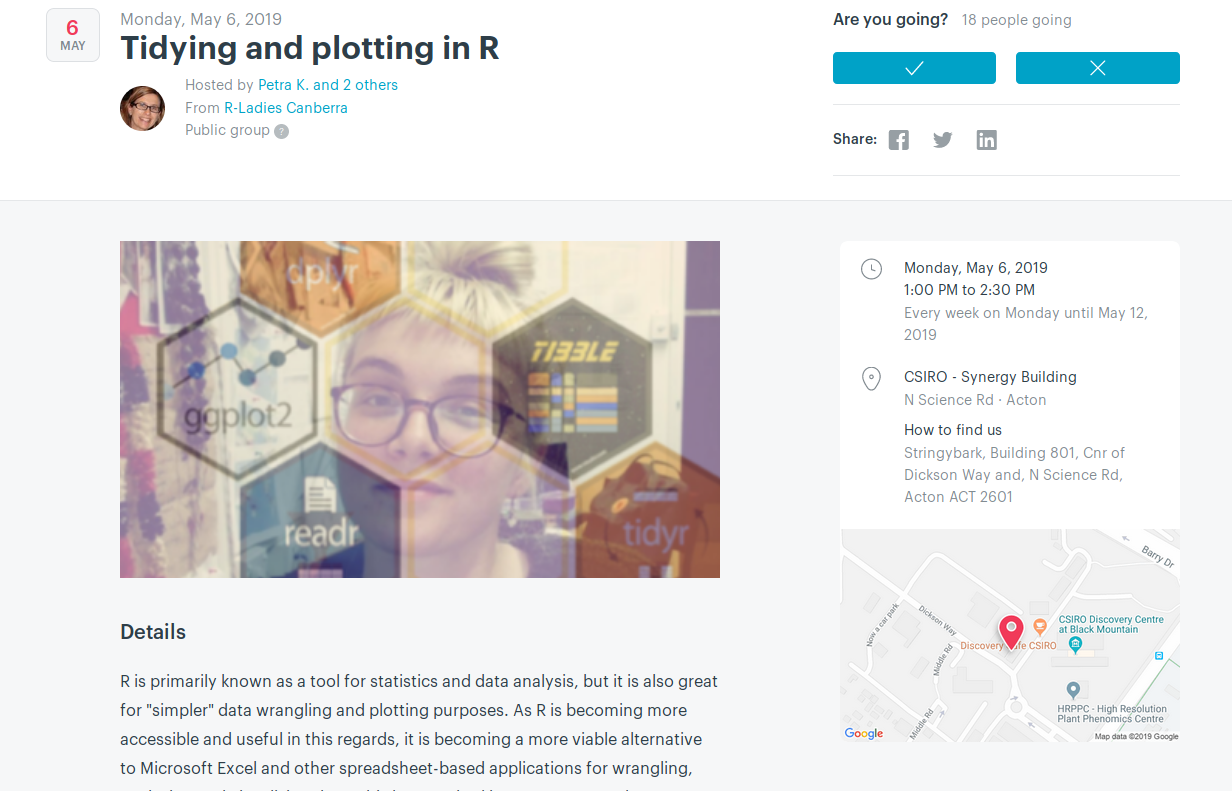
\includegraphics[width=0.9\textwidth]{Figures/rladies.png}

\end{frame}
%%%%%%%%%%%%%%%%%%%%%%%



\begin{frame}{Take-home messages}
  \begin{enumerate}[<+->]
    \item Assumptions are about math properties, but also about scientific logic
    \item In general assumptions are not perfectly met
    \item There are many technics to get closer
    \item "there is no free lunch", every model makes assumptions, explicit or implicit
    \item All models are wrong, a few are useful
  \end{enumerate}
\end{frame}
%%%%%%%%%%%%%

\section{Why we need assumptions}

\begin{frame}{Statistical inference: General approach}

\begin{center}
  \begin{tikzpicture}
    \node (sq) at (0,-1) {\color{red}{1. Scientific question}};
    \pause
      \draw[rounded corners, color=blue] (-4.5,-1.5) rectangle (4,-5.5);
  \node[anchor=north west] (r) at (-4.5,-1.5) {
\includegraphics[width=0.1\textwidth]{Figures/r}};
    \node (mo) at (0,-2) {2. Model and Statistical question};
    \draw[->, thick] (sq)--(mo);
    \pause
    \node (dac) at (6,-2) {\color{red}{3. Data collection}};
    \draw[<->, thick] (mo)--(dac);
    \pause
    \node (est) at (0,-3) {4.a Estimation};
        \draw[->, thick] (mo)--(est);
    \node (unc) at (0,-3.5) {4.b Uncertainty and statistical significance};
    \pause
    
    \node (che) at (0,-5) {5. Prediction, diagnostic, check assumptions};
        \draw[->, thick] (unc)--(che);
    \draw[->, thick, draw=red!80!black, shorten >= 5pt] (che.east) to [out=30, in=330] (mo.east);
    \draw[->, thick, draw=blue!80!black, shorten >= 3pt] (che.east) to [out=70, in=300] (mo.east);
    
    \node (ge) at (6,-4) {\color{red!80!black} Until "good enough"};
    \pause
    \node (ge) at (6,-4.5) {\color{red!80!black} to trust 4.a and 4.b};

    \pause
    \node (int) at (0,-6) {\color{red}{6. Interpret and think about the biology}};
        \draw[->, thick] (che)--(int);


  \end{tikzpicture}
  \end{center}
\end{frame}
%%%%%%%%%%%


\section{What can go wrong; e.g. Linear models}
\begin{frame}[fragile]{Simple linear model}

\centering

  \textbf{{\color{purple}{Response}} = {\color{blue}{Intercept}} + {\color{red}{Slope}} $\times$ {\color{orange}{Predictor}} + {\color{gray}{Error}}} \\

\begin{knitrout}\small
\definecolor{shadecolor}{rgb}{0.843, 0.867, 0.922}\color{fgcolor}
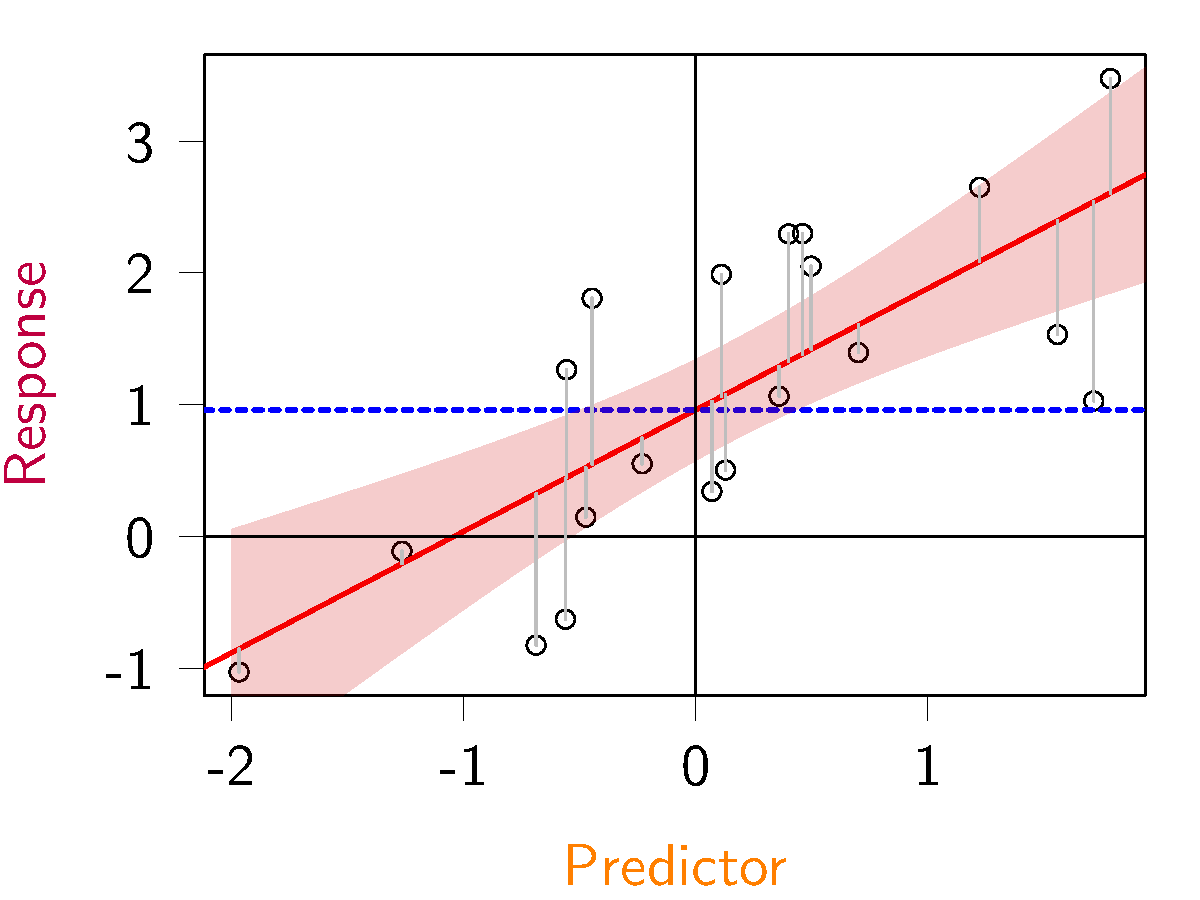
\includegraphics[width=0.8\textwidth,height=0.6\textwidth]{figure/lmprinc-1} 

\end{knitrout}
\end{frame}
%%%%%%%%%%%

\begin{frame}{Linear model assumptions}
\only<1>{\centering \LARGE \textbf{What are linear model assumptions?}}

\only<2>{
  \begin{alertblock}{Assumptions do NOT include:}
  \begin{itemize}
  \item Relationship is a straight line ("Linear" means a line on some scale, not any scale)
  \item Data normality (Only error normality)
  \item Collinearity (Changes parameter meaning, not the validity)
  \end{itemize}
 \end{alertblock}
}
\only<3>{
 \begin{block}{}
     \begin{itemize}
      \item Linear combination of parameters (including transformation, polynoms, interactions\dots)\\ \textit{Risk: biologically meaningless}
      \item Predictor not \textbf{perfectly} correlated \\ \textit{Risk: Model won't run, unstable convergence, or huge SE}
       \item {\color{red!20!black}{Little error in predictors}}\\ \textit{Risk: bias estimates (underestimate with Gaussian error)}
       \item {\color{red!50!black}{Gaussian \textbf{error} distribution}}\\ \textit{Risk: Poor predictions, wrong uncertainty}
       \item {\color{red!70!black}{Homoscedasticity (constant error variance)}}\\ \textit{Risk: Poor predictions, wrong uncertainty}
       \item {\color{red!99!black}{Independence of error}}\\ \textit{Risk: Bias and over-optimistic uncertainty}
     \end{itemize}
 \end{block}
}
 
\end{frame}
%%%%%%%%%%%

\begin{frame}{Residual distributions}
\centering
\textbf{Exercise 1\\ \vfill}
\pause
\textbf{Exercise 2}
\end{frame}
%%%%%%%%%%%


\begin{frame}{Non-independence}
\centering
\textbf{Exercise 3\\ \vfill}
\pause
\textbf{Exercise 4}
\end{frame}
%%%%%%%%%%%

\begin{frame}{Let's think about more complex issues}

\end{frame}
%%%%%%%%%%%

%%%%%%%%%%%%%%%%%%%%%%%%%%%%%%%%%%%%%%%%%%%%%%%%%%%%%%%%%%%%%%%%%%%%%%%%%%%%%
\begin{frame}{Problems / {\color{blue!50}Detection} / {\color{green!50!black}Typical solutions:}}
   \begin{block}{}
     \begin{itemize}[<+->]
      \item Non-Linear relationships / {\color{blue!50} Thinking}\\ \textit{\color{green!50!black}Solution: do you really need that? / non-linear models}
      \item Predictor \textbf{perfectly} correlated / {\color{blue!50} Singular fit}\\ \textit{\color{green!50!black}Solution: Drop redundant variable}
       \item {\color{red!20!black}{Error in predictors}} / {\color{blue!50} Thinking / multiple measurements} \\ \textit{\color{green!50!black}Solution: Better experiment / measurement error model}
       \item {\color{red!50!black}{Non-Gaussian \textbf{error} distribution}} / {\color{blue!50} Plot / experimental design}\\ \textit{\color{green!50!black}Solution: Transformation / GLM}
       \item {\color{red!70!black}{Changing error variance}} {\color{blue!50} Plot / experimental design}\\ \textit{\color{green!50!black}Solution: Transformation / GLM}
       \item {\color{red!99!black}{Correlated errors}} {\color{blue!50} Thinking (/plot)}\\ \textit{\color{green!50!black}Solution: Experimental design / control variables / mixed models}
     \end{itemize}
 \end{block}
\end{frame}
%%%%%%%%%%%%


\begin{frame}{Take-home messages}
  \begin{enumerate}
    \item Assumptions are about math properties, but also about scientific logic
    \item In general assumptions are not perfectly met
    \item There are many technics to get closer
    \item "there is no free lunch", every model makes assumptions, explicit or implicit
    \item All models are wrong, a few are useful
  \end{enumerate}
\end{frame}
%%%%%%%%%%%




\end{document}
